\scanpage{19}\mspage{- IV- \handwritten{1102} -}
(21.6.5) Considérons donc un diviseur \uline{positif} $D^{\unsure{\prime}}$ sur $X$\inserted{ ($X$ é\deleted{\unsure{n}}tant supposé \uline{noethérien})}, de sorte que l'Idéal \inserted{fractionnaire} $\underline I_{X}(D)$ est un \uline{Idéal de} $\underline O_{X}$, qui est un $\underline O_{X}$-Module \uline{inversible}; soit $Y(D)$ le sous-préschéma fermé de $X$ qu'il définit. \deleted{\unsure{Cela signifie}}\inserted{Pour} \deleted{\unsure{qu}} tout $x\handwritten{\in}Y(D)$, \deleted{\unsure{que,}} il y a par hypothèse un voisinage \inserted{\handwritten{ouvert}} $U$ de $x$ dans $X$ et une section \uline{régulière} $t\handwritten{\in\Gamma}(U,\underline O_{X})$ telle que $\underline I_{X}(D)\handwritten{\mid}U=\underline O_{U}\mathbin{.}t$ (21.2.7) ; en d'autres termes, l'immersion canonique $Y(D)\handwritten{\to}X$ est \uline{régulière et de codimension 1} \inserted{(19.1.4) en tout point de $Y( D)$}. On notera d'ailleurs qu'inversement, si $Y$ \reversemarginpar
% slanted
\margin{\figure{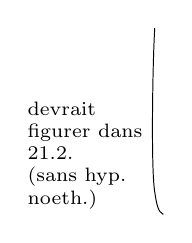
\begin{tikzpicture}[x=1em,y=1em,baseline=0pt]
  \node[anchor=north east,align=left,inner sep=0pt,font=\scriptsize] at (0,0)
    {\handwritten{devrait}\\
     \handwritten{figurer dans}\\
     \handwritten{21.2.}\\
     \handwritten{(sans hyp.}\\
     \handwritten{noeth.)}};
  \draw[line width=.35pt] (.43,2.65) .. controls (.36,1.6) and (.29,-2.25) .. (.42,-3.2)
     .. controls (.49,-3.7) and (.55,-4) .. (.74,-4.08);
\end{tikzpicture}}}
est un sous-préschéma fermé de $X$, régulièrement immergé dans $X$ et \deleted{\unsure{est}} de codimension $1$ en tout point de $Y$, il existe un diviseur positif et un seul \deleted{\unsure{positif}} $D$ sur $X$ tel que $Y(D)=Y$, car\deleted{\unsure{ cela signifie}}\inserted{ pour} \deleted{\unsure{qu}} tout $x\handwritten{\in}Y$, il y a un voisinage $U$ de $x$ dans $X$ tel que $Y\handwritten{\cap}U$ soit défini par un Idéal de $\underline{\mathbb{O}}_{U}$ de la forme $\underline O_{U}\mathbin{.}t$, où $t$ est \uline{réguli\deleted{\unsure{re}}\handwritten{er}} dans $\handwritten{\Gamma}(U,\underline O_{X})$.


Puisque $X$ est supposé noethérien, $Y(D)$ n'a qu'un nombre fini de points maximaux, et en chacun de ces points $x$, on a $\operatorname{codim}(\handwritten{\{}x\handwritten{\}},X)={}\allowbreak{}=\operatorname{dim}(\underline O_{X,x})=1$, autrement dit $x\handwritten{\in}X^{(1)}$ ;
% slanted
\margin{\handwritten{\uline{réf} !}}\normalmarginpar
\deleted{\illegible{2} \unsure{partie} \illegible{1}} en outre, $\underline O_{Y(D),x}$ est un anneau \uline{artinien} en chacun de ces poi\deleted{g}nts. En tout point $x\handwritten{\in}X^{(1)}$ qui n'est pas point maximal de $Y(D)$, on a nécessairement $x\handwritten{\notin}Y(D)$, donc $\underline O_{Y(D),x}=0$. Posons
\[
  \operatorname{cyc}(D)=\handwritten{\sum}^{\handwritten{\prime}}_{x\handwritten{\in}X^{(1)}}
  \operatorname{long}(\underline O_{Y(D),x})\mathbin{.}\handwritten{\overline}{\handwritten{\{}x\handwritten{\}}}
  \tag*{(21.6.5.1)}
\]
qui est donc un élément de $Z^{1}(X)$.

\uline{Proposition} (21.6.6) .- \deleted{\uline{Si} $X$ \uline{est noethérien}}, \uline{\deleted{l}\handwritten{L}'application} $D\handwritten{\leadsto}\operatorname{cyc}(D)$\deleted{\unsure{;}} \uline{est un homomorphisme du monoïde} $\operatorname{Div}^{+}(X)$ \uline{dans} $Z^{1}(X)$ .

Tout revient à voir que pour deux diviseurs \uline{positifs} $D,D'$, on a $\operatorname{cyc}(D+D')=\operatorname{cyc}(D)+\operatorname{cyc}(D')$. Or, on a (21.2.5) $\underline I_{X}(D+D')=\underline I_{X}(D)\underline I_{X}(D')$; tout revient à voir que si $x\handwritten{\in}X^{(1)}$, \inserted{\handwritten{si l'on pose}} $A=\underline O_{X,x}$, et si $t$ et $t'$ sont deux éléments réguliers de $A$, on a $\operatorname{long}(A/tt'A)=\operatorname{long}(A/tA)+{}\allowbreak{}+\operatorname{long}(A/t'A)$ ; mais puisque \deleted{\unsure{$x$}} $t$ est régulier, $tA/tt'A$ est isomorphe à $A/t'A$, d'où \deleted{\unsure{résulte}} aussitôt la proposition.

Il résulte aussitôt des définitions que pour tout ouvert $U\handwritten{\subset}X$, on
% archive sheet number: 18
